
\section{Amodal babble}

Implemented motor "babble" that uses step-wise stochastic search of the control knobs of a motor system, "twiddling" them in a rhythmic fashion.

Then looks for a "resonance" in a specified sensed value (e.g. visual motion, or clear pitch).  This can be very selective to the rhythm - helps discount unrelated events.

Gives automatic method for finding configuration of motor system that produces desired result.


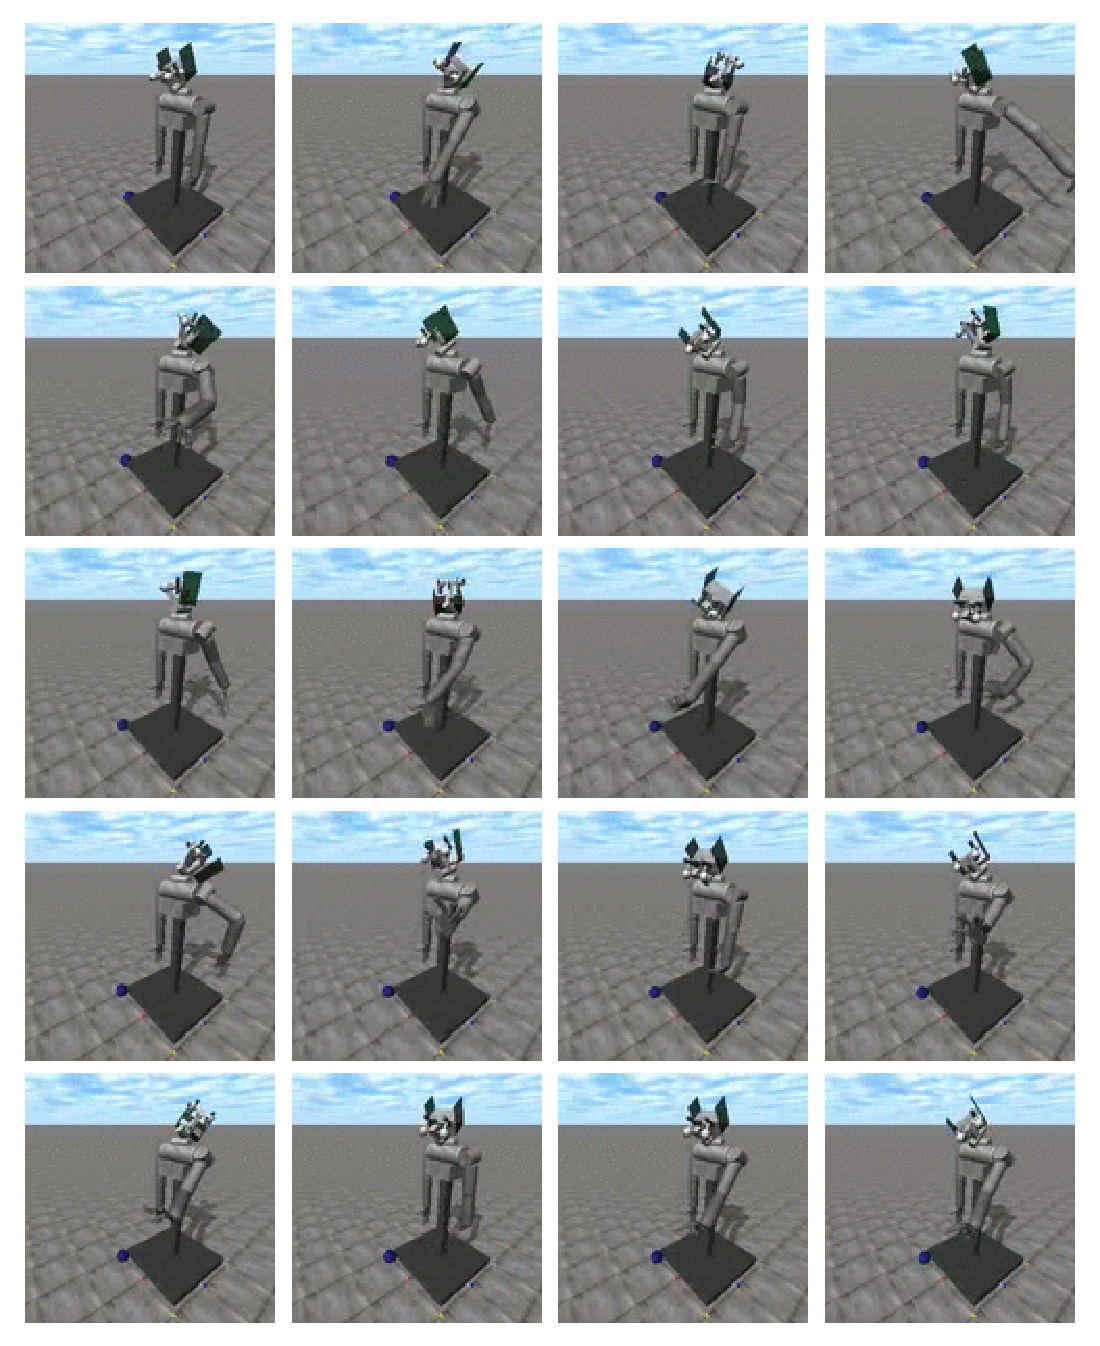
\includegraphics[width=\textwidth]{images/find-arm}


Why?

Want a way of expressing capabilities (such as "bring hand in front of head") in a robust form.

Does NOT assume a tabula rasa - in fact, there is at least as much information involved in exploration (expressing the motor groups to use, their scales, and what sensory cue to monitor) as there would be in just giving numerical pose information.

The difference is robustness to the details of the hand and the head; e.g. could use mirror.

Limitations?

Such stochastic search is very dumb.

Once an initial point of contact has been found, tracking methods would be more efficient for exploring a region of motor space.

Shaking is just one of several amodal cues that could be used (and not a very realistic one)

xref?

Could automate motor space classification examples: gesture recognition, speech recognition

Would have to be a lot simpler than offline, human-mediated work of course.


\subsection{Towards meaning}

The richer the robot's "internal life" is, the more interesting kinds
of "meanings" there can be in its world

- Continuous, broad, shared, structured experience

- Meaning as a process, not a label

Off-line data collection, segmentation, labelling, training of
classifiers, etc work, but restrict the potential semantic universe of
the robot.

For Year 3, online behaviors would be useful.

